\documentclass{Academic}
\usepackage{csquotes}
\usepackage{algorithm}
\usepackage{algpseudocode}

\addbibresource{references.bib}

\begin{document}
%Easy customisation of title page
%TC:ignore
    \myabstract{%\small
%\noindent\textbf{Abstract}
%%Abstract below
%
%The hypothesis/question and its context, scope and significance are briefly and precisely defined. The main conclusions are brief, precise and clear, noting methods used and key results. The language is clear, precise and easy to understand with no irrelevant information.}
    \renewcommand{\myTitle}{Hybrid Recommender Models in E-Learning: A Comprehensive Review of HybridBERT4Rec}
    \renewcommand{\MyAuthor}{Leon Knorr}
    \renewcommand{\MyDepartment}{Mannheim Master of Datascience}
    \renewcommand{\ID}{1902854}
    \renewcommand{\Keywords}{Education, AI, E-Learning}
    \maketitle
%\vspace{-1.9em}\noindent\rule{\textwidth}{1pt} %add this line if not using abstract
    %\onehalfspacing
%TC:endignore

    \section{Introduction}
    In the dynamic landscape of today's knowledge-driven society and global economics, the concept of life-long learning has evolved into a cornerstone for personal and professional development. It ensures the competitiveness of individuals in a globalized market, while also aiding in overcoming social challenges, such as demographic change, social cohesion or public health through continuous education. Because of its key-role in overcoming today's challenges, many governments and corporations invested heavily in lifelong learning offerings and frameworks \cite{rubensonAdultLearningEducation2011}. This investment can be seen by observing the vast landscape of different learning platforms, which have emerged over the last couple of years, ranging from publicly funded E-Learning solutions such as Moodle\cite{StartseiteMoodleOrg} or ILIAS\cite{Ilias}, to private corporate platforms such as Linked-In Learning\cite{LinkedInLearningMit}. As individuals embark on continuous learning journeys on such platforms, the demand for tailored educational experiences has surged. These experiences not only include the recommendation of new content, but also content which aims to aid the user with current learning objectives. Recommender algorithms play a pivotal role in shaping these learning odysseys by providing personalized content recommendations \cite{jeevamolOntologybasedHybridElearning2021}. \\
    In this work, the hybrid content recommendation system HybridBERT4Rec, which uses a transformer based approach to collaborative and content-based filtering techniques, is reviewed and adapted to an E-Learning use case.

    \section{Related Work}

    \section{Sequential Content Recommendation}\label{sec:seq_recom}
    Traditional content recommendation systems usually observe user interactions as a set of independent and unrelated data points. These systems then compute or form a hidden representation in order to model user interests, which can then be used to predict which items may be relevant for the given user. If an item is considered relevant, it gets recommended. This modeling technique models a user's \textit{general} preferences and interests \cite{wangSequentialRecommenderSystems2019}. But, this is insufficient modelling, as user preferences change over time \cite{wangSequentialRecommenderSystems2019}! For example, let Alice be a user whose general interests reflect romantic films, such as Titanic, Romeo \& Juliet or \enquote{me before you} and who recently got into the Marvel Universe, and started watching Movies like \enquote{Spider-Man}. In addition, Alice is now really interested in following up with that series. Alice's movie history contains a total of 10 movies, 9 romantic movies and one Spider-Man movie, with the latter being the most recently watched. A traditional content recommendation system would observe Alice's movie history and model her interests as consisting of 90\% romantic films and 10\% Marvel. As a result, the recommendation system would assign romantic films a higher relevance score than a movie that is similar to Spider-Man, leading to unsatisfying recommendations for Alice's \textit{current} interests. Sequential Content Recommendation aims to solve this problem by observing user-interactions as a sequence. Thus, these models not only consider the items in the user history, but also the temporal aspect given by the order in which the items occur \cite{wangSequentialRecommenderSystems2019}. This ordering implies that more recent interactions are more relevant for recommending the next item, but at the same time also covers a user's general interest. As a result, Sequential Recommendation models are able to make accurate recommendations at any point in time, that also reflect temporary spikes of interests, while at the same time being able to recommend content that the user may generally be interested in. By choosing sequences as their data model, these models also gain a lot of flexibility in terms of the use cases they are able to cover. Because Sequential Recommendation models do not predict the relevance of items directly, but predict user-interaction probabilities at a given time-step, they are able to not only make recommendations for the present, but also for the future \cite{wangSequentialRecommenderSystems2019}. This allows these models to predict sequences of items, which can be used to craft recommendation series. E.g. a movie recommendation system can then recommend a complete series of movies which fit to Alice's interest in Marvel films, by predicting not only the next movie the user is likely to interact with but the next $n$ movies. These reasons, render Sequential Recommendation models theoretically superior to traditional recommendation models in terms of content recommendation. \\
    \begin{figure}[ht!]
        \centering
        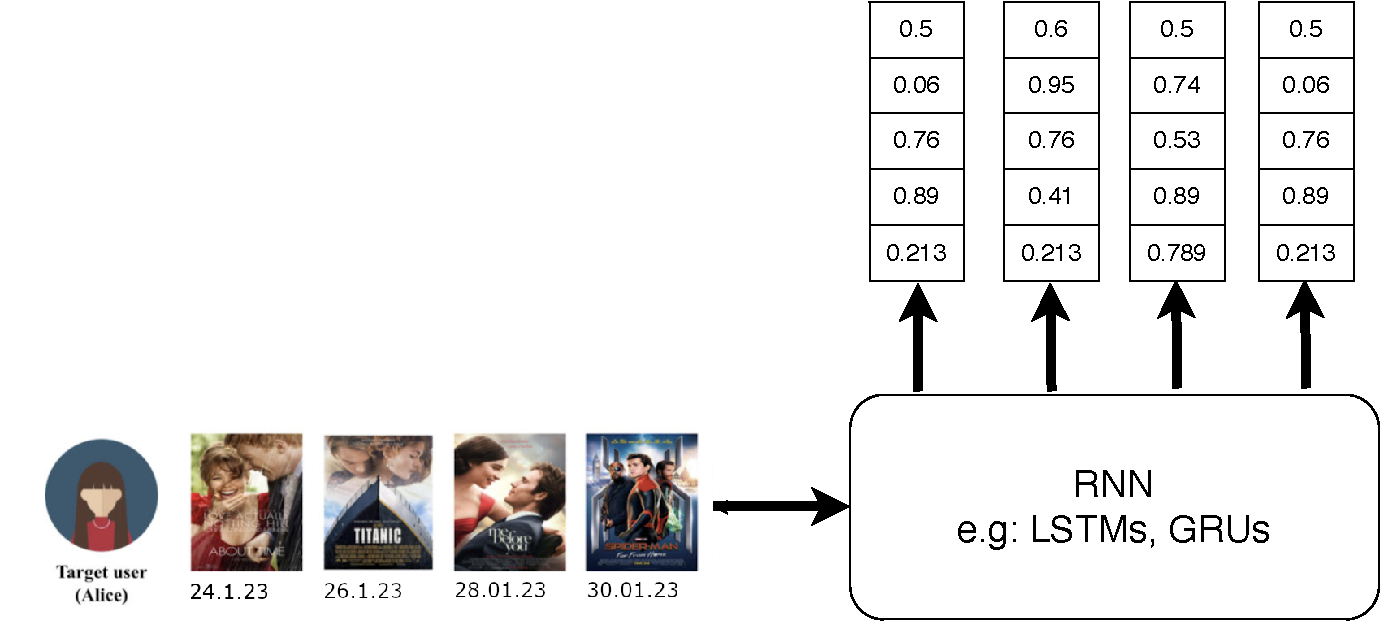
\includegraphics[width=0.6\textwidth]{images/rnn_seq.pdf}
        \caption{Sequential Content Recommendation with RNNs \cite{yuDynamicRecurrentModel2016}}
        \label{fig:seqRNN}
    \end{figure}
    A common approach to realizing Sequential Recommendation models is by using Recurrent Neural Networks (RNNs), such as Long-Short-Term-Memory (LSTMs) or Gated-Recurrent-Units (GRUs), as depicted in Figure \ref{fig:seqRNN}. The RNN gets the sequence of user-interactions or items as input, in this case movies, and encodes them into a fixed length vector representation, which gets updated at every time-step in the sequence. The model then predicts the interaction probabilities or rating scores for every item which may be recommended at the next time step \cite{yuDynamicRecurrentModel2016}. An example, for such an application can be found in Fung Yu et al. DREAM model \cite{yuDynamicRecurrentModel2016}. However, these models suffer from common RNN problems, such as catastrophic forgetting, vanishing gradients and uni-directionality, as well as their inefficiency when dealing with longer sequences. This motivates the use of transformer based models, more specifically HybridBERT4Rec, which allows to use a sequence based approach to content recommendation without the downsides of RNNs \cite{channarongHybridBERT4RecHybridContentBased2022}.

    \FloatBarrier

    \section{HybridBERT4Rec}
        \begin{figure}[ht!]
            \centering
            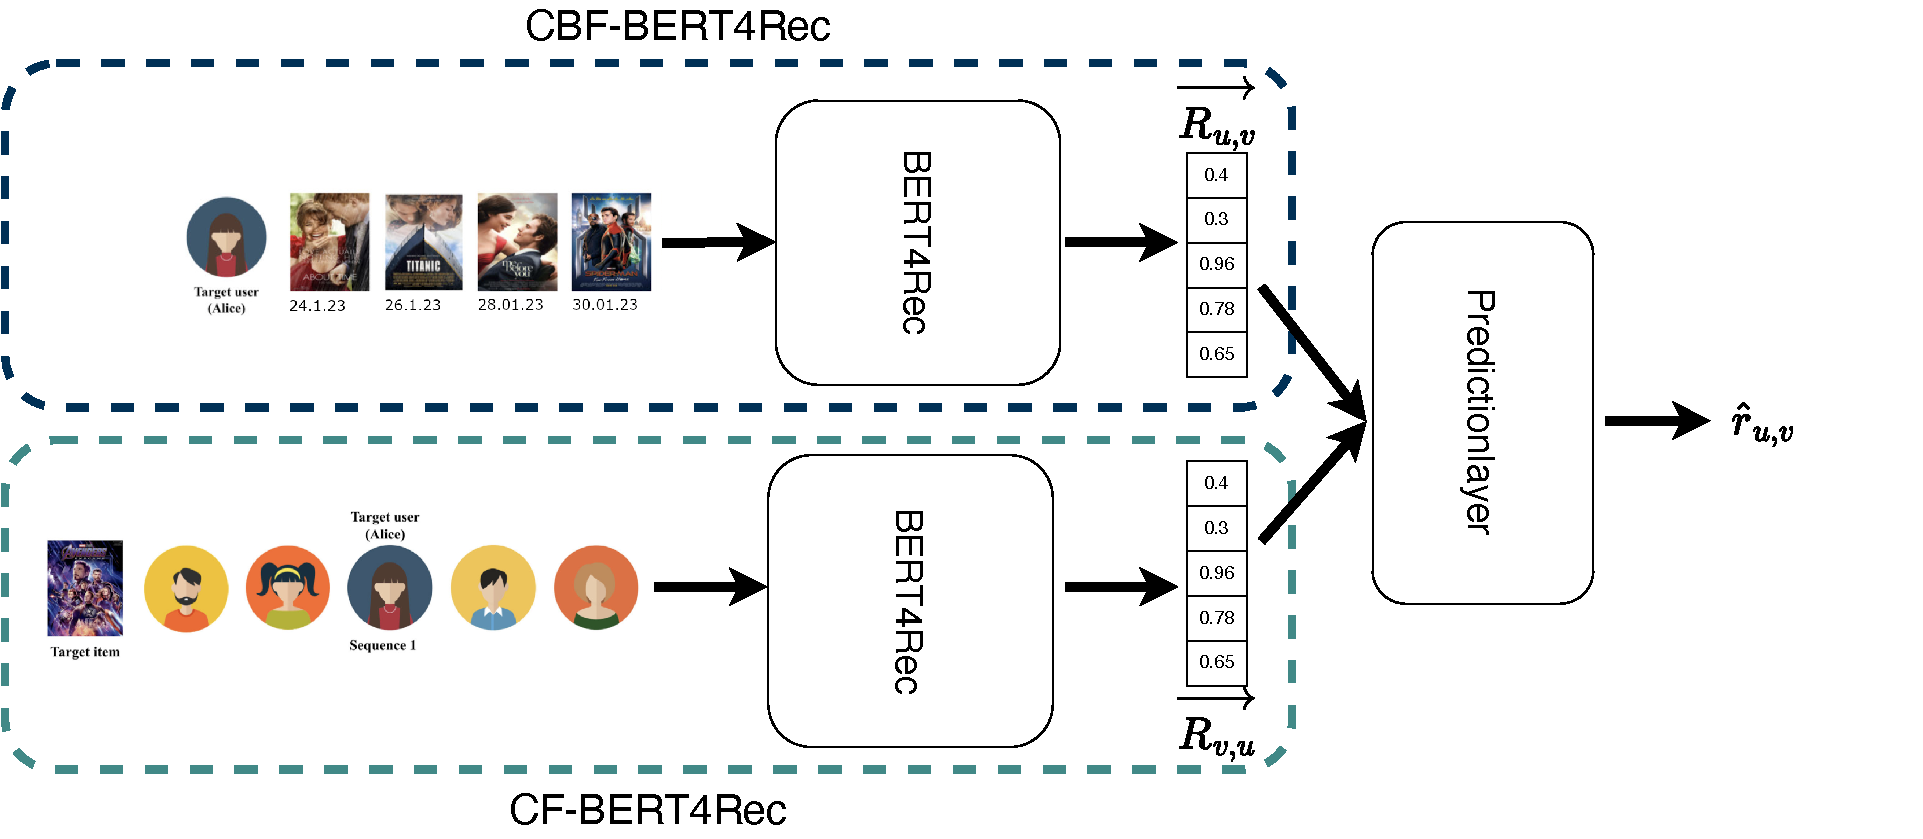
\includegraphics[width=0.6\textwidth]{images/hybridBERT4Rec_high_level.pdf}
            \caption{High level overview of HybridBERT4Recs Architecture. \cite{channarongHybridBERT4RecHybridContentBased2022}}
            \label{fig:highlevel}
        \end{figure}
        HybridBERT4Rec is a hybrid recommendation model, which was originally developed by Chanapa Channarong et al. \cite{channarongHybridBERT4RecHybridContentBased2022} on a movie recommendation task \cite{channarongHybridBERT4RecHybridContentBased2022}. It uses a combination of Collaborative Filtering (CF) and Content Based Filtering (CBF) methods, in order to predict a relevance score for a given target item.
        As shown in Figure \ref{fig:highlevel}, it consists of three main parts:
        \begin{enumerate}
            \item CBF-BERT4Rec: Models Content Based Filtering
            \item CF-BERT4Rec: Models Collaborative Filtering
            \item Prediction layer: Combines both approaches and predicts the final relevance score $\hat{r}_{u,v}$
        \end{enumerate}
        Both the CBF- and CF-Part of the model build upon HybridBERT4Recs predecessor BERT4Rec, and use the exact same architecture, while working with different inputs, in order to model their respective filtering techniques.

        \subsection{BERT4Rec}\label{seq:bert4rec}
        \begin{figure}[ht!]
            \centering
            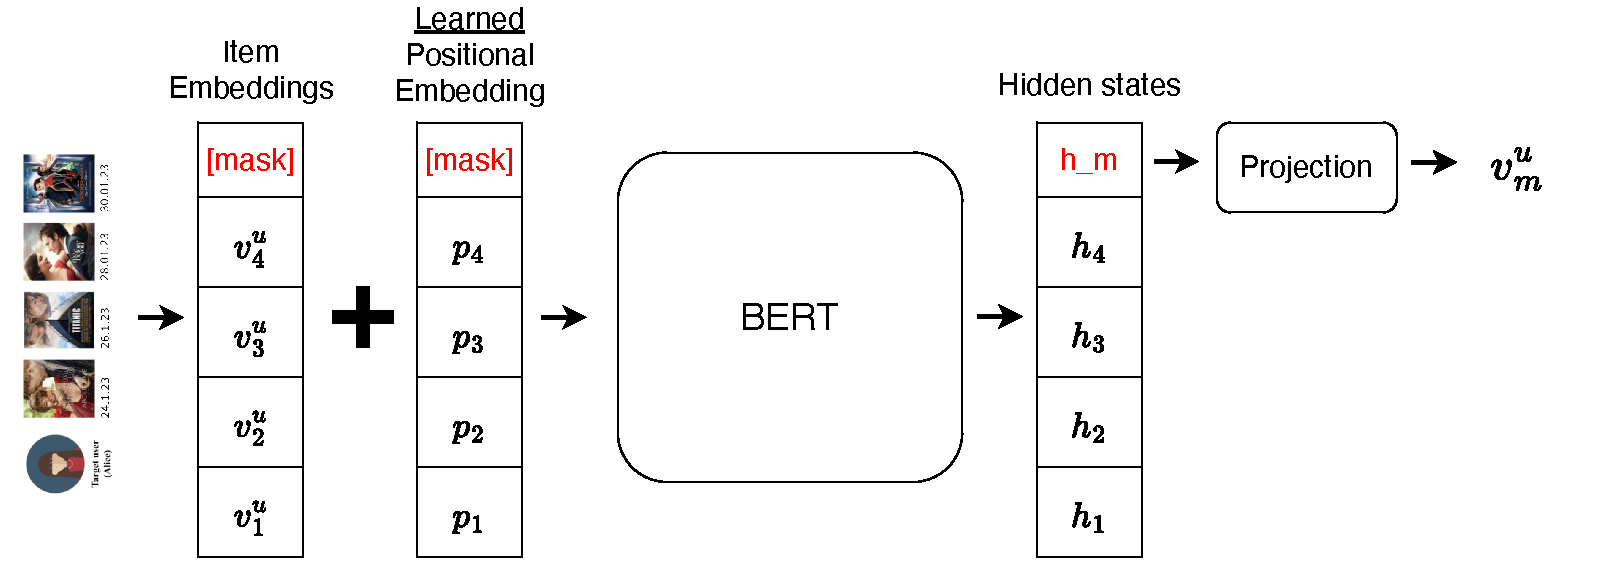
\includegraphics[width=0.6\textwidth]{images/BERT4Rec.pdf}
            \caption{BERT4Rec Architecture, taking item embeddings $v_t^u$ from user $u$'s history as input and predicts the next item $v_m^u$, u is likely to interact with \cite{sunBERT4RecSequentialRecommendation2019}.}
            \label{fig:bert4rec}
        \end{figure}
        BERT4Rec is a content recommendation model, which is based on the Bidirectional Encoder Representations from Transformers (BERT) model in order to facilitate Content Based Filtering. It has been developed in order to predict the next item a user is likely to interact with from a sequence of item embeddings from a user's interaction history. As depicted in Figure \ref{fig:bert4rec} The model consists of a learned positional embedding layer, an unmodified BERT transformer and a projection layer. In order to train BERT4Rec, Fei Sun et al. \cite{sunBERT4RecSequentialRecommendation2019} applied Masked Language Modelling, a common training technique from Natural Language Processing and transferred it to the domain of recommendation models. As a result, during training, one or more items in the input sequence are masked at random and replaced with a special \texttt{[mask]} token. Then, the learned positional embeddings are added to the item embeddings, and the sequence gets passed on to the standard BERT transformer. The resulting hidden representation, of the masked item(s) is then passed through the prediction layer, which consists of a two layer feed forward neural network with GELU activations and a softmax layer, as given by equation \ref{eq:pred_bert4rec}. This layer then produces an output distribution over the target items the model is supposed to rank.
        \begin{equation}\label{eq:pred_bert4rec}
            P(v) = \mathrm{softmax}(\texttt{GELU}(h_t^LW_p+b_p)E_T + b_O) \text{\cite{sunBERT4RecSequentialRecommendation2019}}
        \end{equation}
        In Equation \ref{eq:pred_bert4rec}, $h_t^L$ marks the hidden representation of the masked token, $W_p$ is the weight matrix of the linear layer, $b_p$ and $b_O$ are bias terms and $E_T$ is the item embedding matrix, which is also used to convert the items in the input sequence to item embeddings. The embedding matrix was reused in order to alleviate overfitting and reduce model size \cite{sunBERT4RecSequentialRecommendation2019}. \\
        This training objective allows the transformer to learn strong and meaningful item representations from their contexts. In the domain of recommendation models, this translates to learning how to construct the item representation of the next optimal item a user would want to interact with from the user's history. The prediction layer then essentially calculates similarity scores between this optimal item representation and the target items.\\
        Despite its upsides, using BERT4Rec in a standalone manner, still comes with a limitation. As the prediction is solely based on extracting user historical patterns which can be seen as characteristics the user favors, the model can't recommend items from categories that aren't included in the user history already. In other words, it can't help a user discover new content, which is a general downside of using CBF in a standalone setting \cite{channarongHybridBERT4RecHybridContentBased2022}. HybridBERT4Rec overcomes this issue by taking a hybrid approach to content recommendation by not only focusing on CBF but also using Collaborative Filtering techniques. But, before presenting how HybridBERT4Rec achieves Collaborative Filtering, the usage of BERT4Rec is put into context by laying out how HybridBERT4Rec achieves CBF using BERT4Rec in the following subsection.

        \subsection{CBF-BERT4Rec}
        \begin{figure}[ht!]
            \centering
            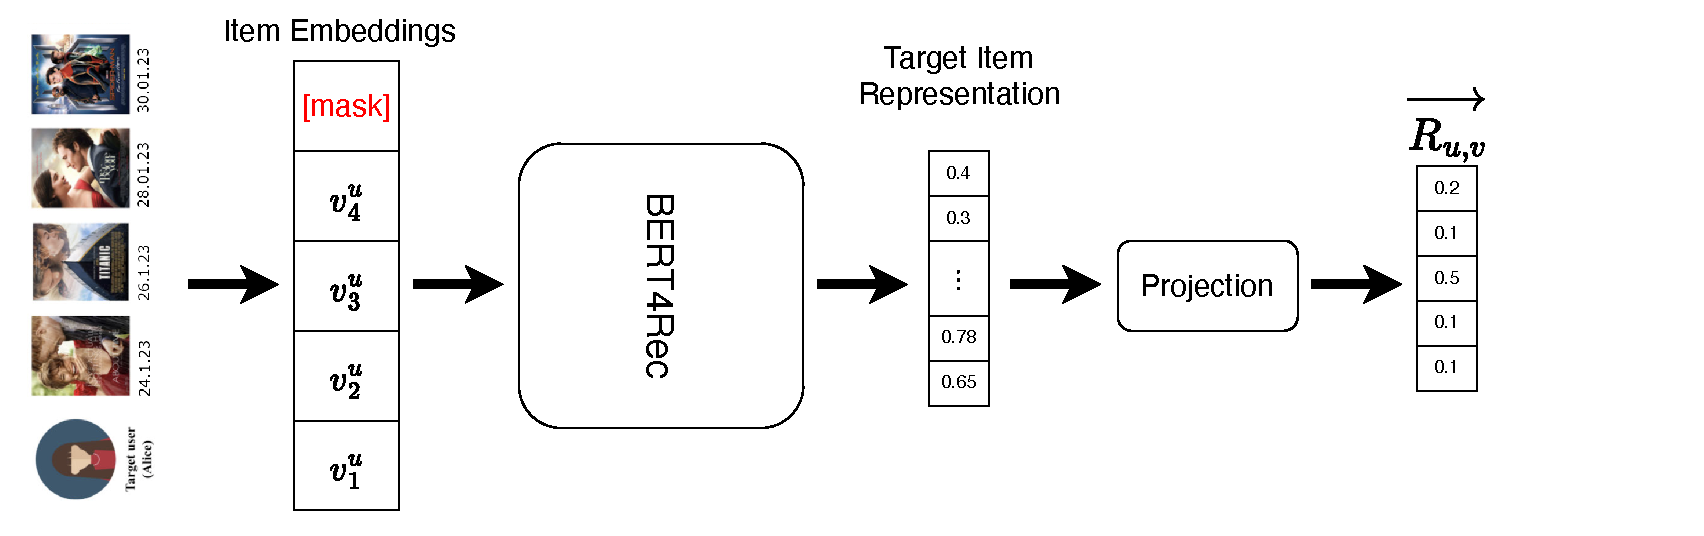
\includegraphics[width=0.6\textwidth]{images/CBF-HybridBERT4Rec.pdf}
            \caption{CBF-HybridBERT4Rec Architecture, taking item embeddings from a user $u$ history as input and predicts a \enquote{target user profile $\overrightarrow{R_{u,v}}$} \cite{channarongHybridBERT4RecHybridContentBased2022}.}
            \label{fig:cbf-arch}
        \end{figure}
        As laid out earlier, the responsibility of CBF-BERT4Rec is to realize Content Based Filtering. In other words, it aims at extracting the target user representation, which describes the users preferences and interests. As shown in Figure \ref{fig:cbf-arch}, it achieves this by deploying BERT4Rec directly without any modifications. The input to the model is then given by the sequence of items in the target users history in chronological order. Then random item(s) are masked during the training process, during inference, the \texttt{[mask]} token is appended to the sequence and the model calculates the hidden representation for the masked token. This representation is then passed through the projection layer, as described earlier. The resulting distribution is then a distribution of all items over the \enquote{optimal item}, expressed as the interaction probability of the target user with all items. Chanapa Channarong et al. \cite{channarongHybridBERT4RecHybridContentBased2022} call this distribution the \enquote{target user profile $\overrightarrow{R_{u,v}}$}
        \FloatBarrier

        \subsection{CF-BERT4Rec}\label{sec:cf_bert4rec}
        In order to overcome the aforementioned limitations of only using CBF, HybridBERT4Rec also uses CF techniques. Implementing CF is the main responsibility of the CF-BERT4Rec part of HybridBERT4Rec. CF-BERT4Rec achieves collaborative filtering by constructing the representation of a target item based on the target user and its set of neighbors. As shown in Figure \ref{fig:cf-arch}, it also deploys BERT4Rec unmodified similar to CBF-BERT4Rec, but it uses completely different data. The input to CF-BERT4Rec is constructed by creating a sequence of all users who have interacted with the target item in chronological (in the case of movies, this is equivalent to all users who have rated the target movie). This may or may not include the target user. Again during inference, the \texttt{[mask]} token is appended to the sequence, and it is passed through BERT4Rec. The model will then construct a representation of the target item, reflecting the \enquote{optimal user} for this item, based on the neighboring users in the user sequence, which is passed on to the prediction layer. The prediction layer then yields a distribution of all neighboring users over the \enquote{optimal user}, expressed as user-similarity probabilities between the neighboring users and the target user, which is also called the \enquote{target item profile $\overrightarrow{R_{v,u}}$} \cite{channarongHybridBERT4RecHybridContentBased2022}.
        \begin{figure}[ht!]
            \centering
            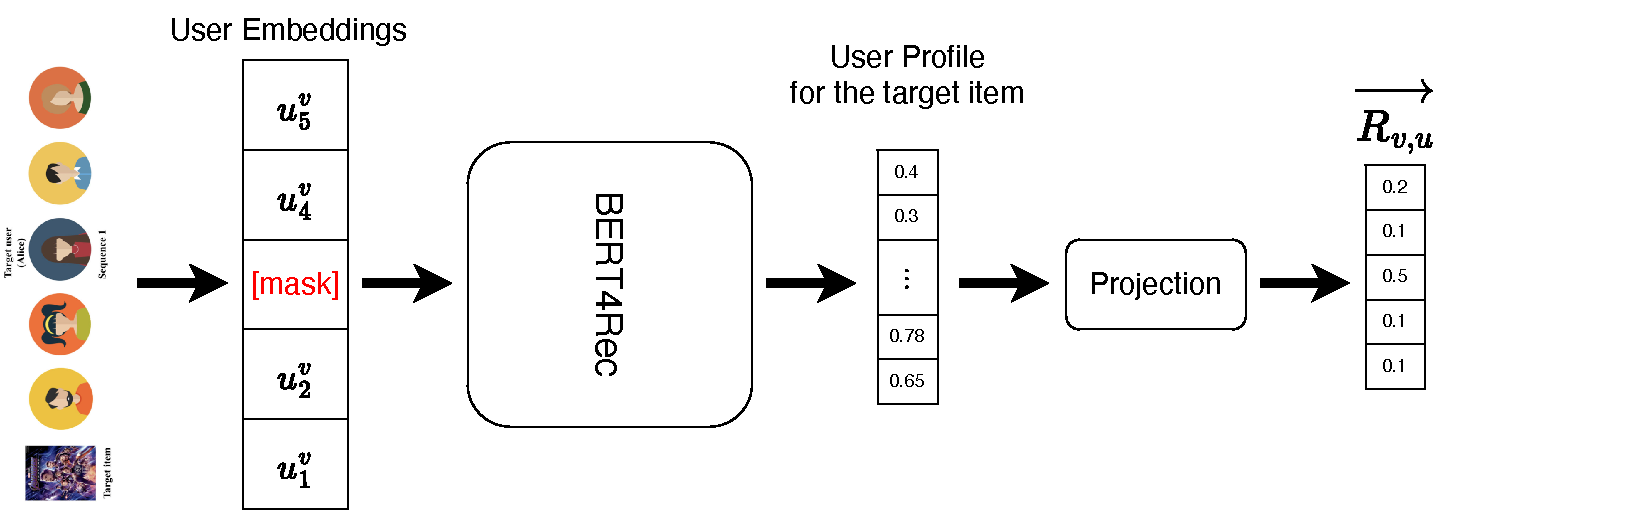
\includegraphics[width=0.6\textwidth]{images/CF-HybridBERT4Rec.pdf}
            \caption{CF-HybridBERT4Rec Architecture, taking user embeddings from all users that have rated the target item $v$ as input and predicts the \enquote{target item profile $\overrightarrow{R_{v,u}}$} \cite{channarongHybridBERT4RecHybridContentBased2022}.}
            \label{fig:cf-arch}
        \end{figure} \\
        This approach to collaborative filtering is quite unusual, as modeling the \textit{set} of neighbors as a sequence is questionable. The argument that the set of neighbors change over time and some might be more important than others does not hold in the same way as with content based filtering in collaborative filtering. Even though a users preferences might change overtime, and thus his current interests might not match with his past interests anymore, and he might thus not be a close neighbor anymore, his inclusion in the set of neighbors with an equal weighting is still valid. The reason for this is, that the primary goal of the inclusion of Collaborative Filtering is to enable \textit{exploration}. The recommender system is supposed to help the user explore new content by sacrificing the overall precision of the recommendations. Thus, the user who has moved from his past interests, is still as important as before, as the target user might be interested in following this user's direction as the system might not be aware of a specific interest of the target user. Because of that, the inclusion of a transformer based model in this case is questionable, as collaborative filtering in general only requires the calculation of user-user similarities between neighbors and the target user \cite{channarongHybridBERT4RecHybridContentBased2022}. As a result, the collaborative filtering part could have been implemented with a smaller and more efficient model, than with BERT4Rec. The authors also don't provide much reasoning as to why the use of a transformer based sequence recommendation model is beneficial for collaborative filtering \cite{channarongHybridBERT4RecHybridContentBased2022}.

        \subsection{Prediction Layer}
        % \begin{figure}[ht!]
        %     \centering
        %     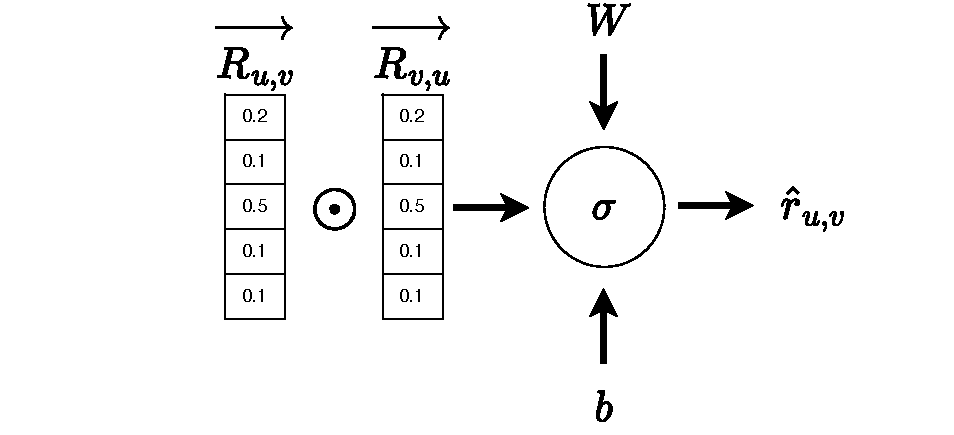
\includegraphics[width=0.5\textwidth]{images/Prediction_Layer.pdf}
        %     \caption{Schematic of HybridBERT4Recs Prediction layer, which uses a generalization of Matrix Factorization based on Neural Networks with Sigmoid activations to predict the rating $\hat{r}_{u,v}$ user $u$ would assign to item $v$ \cite{channarongHybridBERT4RecHybridContentBased2022}.}
        %     \label{fig:pred_layer}
        % \end{figure}
        The last layer in HybridBERT4Rec is the Prediction Layer. It combines the target item profile $\overrightarrow{R_{v,u}}$ from the CF-part with the target user profile $\overrightarrow{R_{u,v}}$ from the CBF-part of the model through Generalized Matrix Factorization (GMF), in order to predict a final relevance score $\hat{r}_{u,v}$, which target user $u$ would assign to the target item $v$. The computation performed by this layer is given by Equation \ref{eq:pred_layer}, where $\odot$ denotes the element-wise product of both vectors \cite{channarongHybridBERT4RecHybridContentBased2022}.
        \begin{equation}\label{eq:pred_layer}
            \hat{r}_{u,v} = \sigma(WR(u,v) + b), \text{ with }
            R(u,v) = R_{uv} \odot R_{vu}
        \end{equation}
        In contrast to traditional Matrix Factorization, generalized matrix factorization is based on neural networks with sigmoid activations, which are trained with a log-loss. This allows the model to learn the interaction function between the user- and item profile from data. This grants the model the ability to express a form of Matrix Factorization that isn't uniform and non-linear. In other words, it is able to assign different weights to different latent dimensions of the user-item vector $R(u,v)$ and is able to model non-linear and more complex structures than traditional Matrix Factorization \cite{heNeuralCollaborativeFiltering2017}.

        \subsection{Strengths \& Weaknesses}
        This transformer based architecture comes with several strengths:
        \begin{enumerate}
            \item \textbf{Highly parallelizable:} The model can be efficiently parallelized in several ways. First, it inherits the sequential in depth characteristics of transformer models. This means that the models internal computations can be efficiently parallelized on a per-layer basis, as the computation for time step $t$ at layer $l$ is independent of the result of the computation for time step $t+1$ or $t-1$ at layer $l$.
            \item \textbf{Bi-directionality:} Because HybridBERT4Rec is based on BERT, it inherits BERTs Bi-directionality. This allows the model to compute more expressive and meaningful representations of items, as these representations are not only dependent on past contents ($t < t_{present}$) but also on future ($t > t_{present}$) contents, providing a more sophisticated and information rich context for each token in the input sequence.
            \item \textbf{Sequential modelling:} It inherits the strengths of sequential content recommendation models, as explained in Section \ref{sec:seq_recom}. However, as layed out in Section \ref{sec:cf_bert4rec}, the use of a sequential approach to Collaborative Filtering remains questionable.
            \item \textbf{Independent Execution \& Caching:} HybridBERT4Recs CF- and CBF-part can be executed independent of each other, as no data flow is required between both parts. If this is combined with the ability to cache the target item- and user- profiles, then the model allows for dynamic profile calculations whenever needed. For example, it is only necessary to calculate the target user profile once for each item and similarly, the target item profile once for each user, as long as there is no update to either of them. If an update to one of them occurs, for example user $u$ watches a movie, and it is appended to his history, then \textit{only} the target item profile for user $u$ needs to be updated. There is no need to run the model for every user and every item again. At recommendation time, the cacheability of the user- and item-profiles also reduces the models time and hardware requirements, as only the comparatively small and shallow prediction-layer needs to be executed in order to retrieve new recommendations. Both, independent execution and caching grant the model a high flexibility in terms of model deployment and applications.
        \end{enumerate}
        Despite its numerous strengths, the model also includes some significant weaknesses:
        \begin{enumerate}
            \item \textbf{Limited Sequence Length:} Inheriting the characteristics of transformer models also means inheriting their weaknesses, in particular the limited sequence length. Because the per-layer complexity of the self-attention mechanisms of $O(n^2*d)$, where $n$ denotes the sequence length and $d$ the representation dimension, self-attention architectures scale badly in terms of sequence length \cite{vaswaniAttentionAllYou2017}. This combined with memory constraints of modern hardware limits the sequence length of any transformer based model. In the domain of recommendation systems, this translates to limiting the maximum length of user histories, and potential neighbors to form both the target user- and target item profiles. In the case of the movie recommendation example, used throughout this paper, it limits the length of a users watch history and the maximum number of ratings that can be taken into consideration in order to form a user's potential neighbors.
            \item \textbf{Hardware Requirements:} Because of HybridBERT4Recs hybrid nature, combining both Collaborative Filtering and Content Based Filtering, it also uses two seperate BERT based transformer models to model each approach. In the worst case, this translates to executing a transformer model for each of our users, another transformer model for each of our items and the prediction layer for each user-item combination, \textit{if intermediate results are cached}! If no caching is present, both transformer models and the prediction layer would have to be executed \textit{for every user and item combination}. In both cases, the model requires lots of processing power and memory in order to run. However, both processing and memory requirements do decrease significantly if the aforementioned optimization opportunities for dynamic recalculations, independent execution and caching are used. In addition, transformer models need comparatively large datasets if trained from scratch \cite{channarongHybridBERT4RecHybridContentBased2022,sunBERT4RecSequentialRecommendation2019,vaswaniAttentionAllYou2017}.
        \end{enumerate}

        \subsection{Performance \& Experiments}
        Chanapa Channarong et al. \cite{channarongHybridBERT4RecHybridContentBased2022} evaluated HybridBERT4Rec on three different datasets:
        \begin{itemize}
            \item MovieLens1M \cite{MovieLens1MDataset2015}: A movie recommendation dataset aimed at building and evaluating recommendation algorithms. It is composed of one million ratings from 6000 users on 4000 movies, with each user being responsible for at least 20 ratings.
            \item Yelp \cite{YelpDataset}: A dataset consisting of eight million ratings of restaurant and service business reviews, where each user created at least four ratings.
            \item GoodReads \cite{wanFineGrainedSpoilerDetection2019}: A book review dataset consisting of one million ratings, where each user has been responsible for at least 70 ratings.
        \end{itemize}
        As evaluation metrics, they adopted the Hit Ratio (HR) of the top $k$ predictions, which measures the ranking accuracy, and the Normalized Discounted Cumulative Gain (NDCG), which measures the recommendation list quality of the top $k$ positions. Along HybridBERT4Rec, they reported the performance of four additional models:
        \begin{itemize}
            \item Caser \cite{tangPersonalizedTopNSequential2018}: Caser is a unidirectional CBF approach using Convolutional Neural Networks (CNNs), which predicts the top-$N$ ranked items that a user will likely interact with.
            \item GRU4Rec \cite{hidasiSessionbasedRecommendationsRecurrent2016}: GRU4Rec is a unidirectional CBF approach using Recurrent Neural Networks (RNNs), more specifically Gated Recurrent Units, which predicts the next item embeddings at every time step.
            \item SAS4Rec \cite{kangSelfAttentiveSequentialRecommendation2018}: SAS4Rec is a unidirectional CBF approach, which uses a transformer-based architecture to predict the next item a user will interact with.
            \item BERT4Rec \cite{sunBERT4RecSequentialRecommendation2019}: As covered in Section \ref{seq:bert4rec}, it is a bidirectional transformer based architecture, which predicts the next item a user is likely to interact with. 
        \end{itemize}
        The results for NDCG@50 reported by Chanapa Channarong et al. \cite{channarongHybridBERT4RecHybridContentBased2022} are depicted in Figure \ref{fig:perfExp}.
        \begin{figure}[ht!]
            \centering
			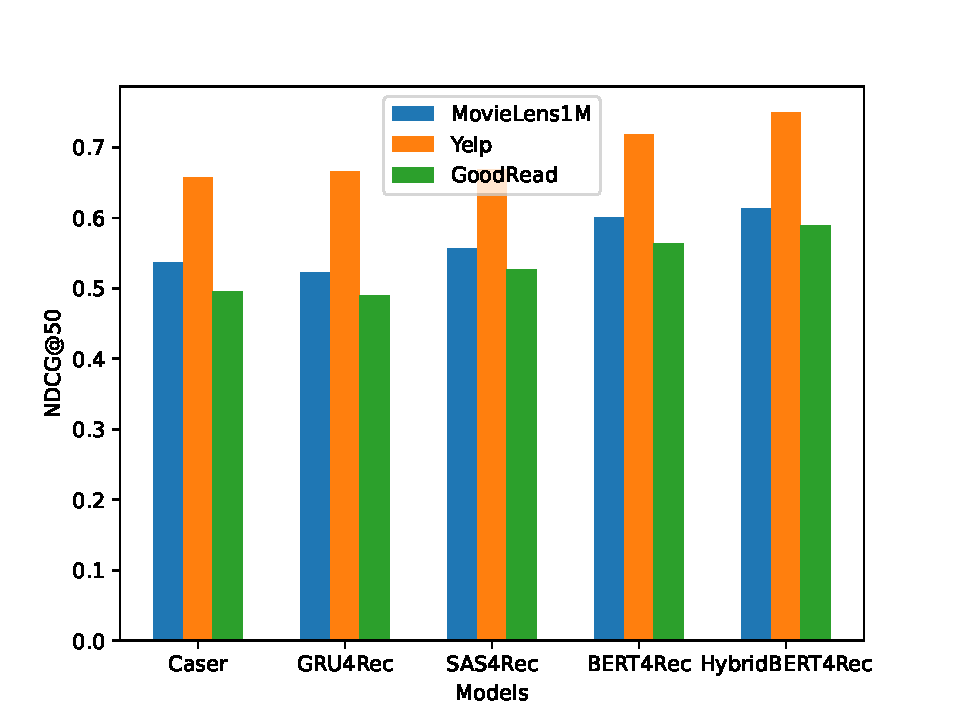
\includegraphics[width=0.6\textwidth]{images/results.pdf}
			\caption{Performance comparison of different recommender models on three datasets as published by the authors of HybridBERT4Rec \cite{channarongHybridBERT4RecHybridContentBased2022}.}
            \label{fig:perfExp}
		\end{figure}
        In their experiments, HybridBERT4Rec outperforms all other models across all three datasets, with BERT4Rec being the second-best model and Caser performing the worst. The same result was obtained for the HR and all other values of $k$ for both metrics, hence these results haven't been directly reported in this paper again. For a detailed look at the numbers, please refer to Channarong et al. original paper \cite{channarongHybridBERT4RecHybridContentBased2022}. The results reported are not surprising, given that the \textit{Hybrid} bidirectional HybridBERT4Rec model was evaluated solely against unidirectional (except for BERT4Rec) \textit{Content Based Filtering} models. With that, the experiments are not representative in order to evaluate HybridBERT4Rec performance. The main takeaways presented by the experiments are that BERT4Recs bidirectional approach performs better than its unidirectional competitors and that the inclusion of Collaborative Filtering into Content Based Filtering models is effective and can increase recommendation performance. But, it remains unclear how HybridBERT4Rec performs in comparison to other hybrid recommendation models.\\
        In addition, the authors don't provide much information about how the data for training and testing has been partitioned for these experiments. They mention, that some authors had to be pruned from the datasets, because their histories were too short for model training, but other than that, no further information is provided. As a result, HybridBERT4Recs generalization performance also remains unknown, along with questions like: Does it suffer from the cold start problem? How does it handle new and unseen items / users? How does it handle domain transfer after training? Does it inherit the fine-tuning capabilities transformers are well known for \cite{radfordImprovingLanguageUnderstanding}? Without these questions answered the real world applicability of this model is unknown, as it is unclear how it would handle such a dynamic and fast-paced environment.

    \section{Applying HybridBERT4Rec in an E-Learning Environment}

        \subsection{The Trivial Solution}
        \begin{figure}[ht!]
            \centering
			
\includegraphics[width=0.3\textwidth]{images/linked_in_landing.pdf}
            
\includegraphics[width=0.3\textwidth]{images/linked_in_course.pdf}
			\caption{Linked-In Learning landing-page and course overview \cite{LinkedInLearningMit}.}
            \label{fig:trivSol}
		\end{figure}
    
        \subsection{The Setting}
    \begin{figure}[ht!]
        \centering
        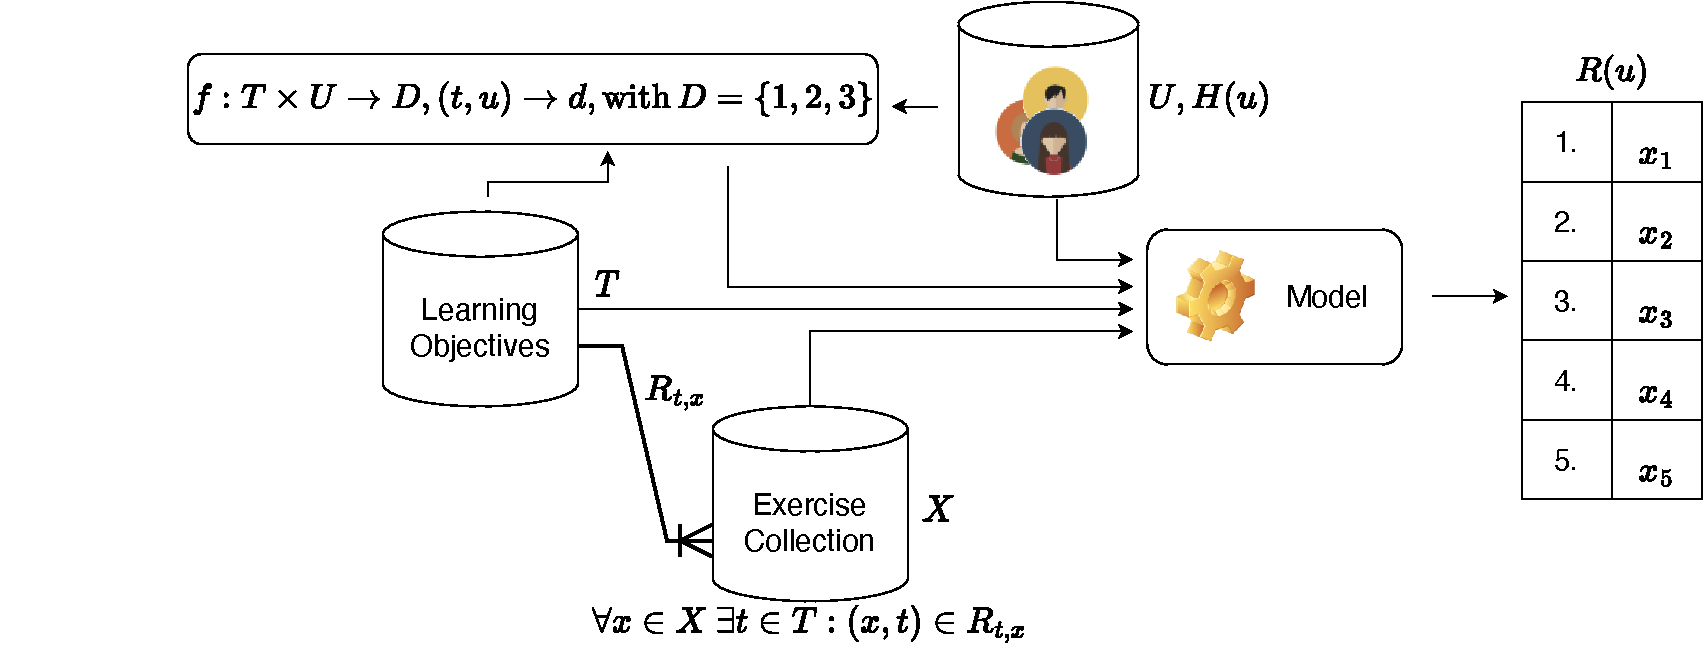
\includegraphics[width=0.6\textwidth]{images/setting.pdf}
        \caption{The Setting, consisting of a user collection $U$ and their histories $h(u)$, a collection of learning objectives $T$ and a collection of exercises $X$, which can be used to predict a ranking $R(u)$ for a given user $u$.}
        \label{fig:setting}
    \end{figure}

    \subsection{Model Adaption}
    \begin{figure}[ht!]
        \centering
        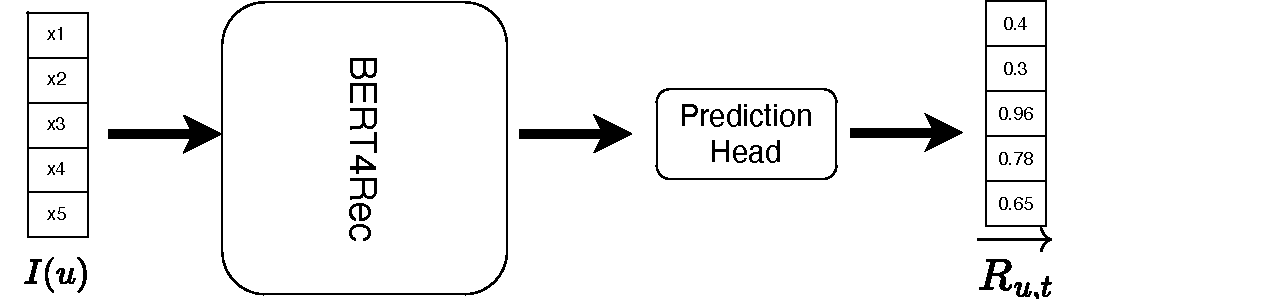
\includegraphics[width=0.4\textwidth]{images/cbf.pdf}
        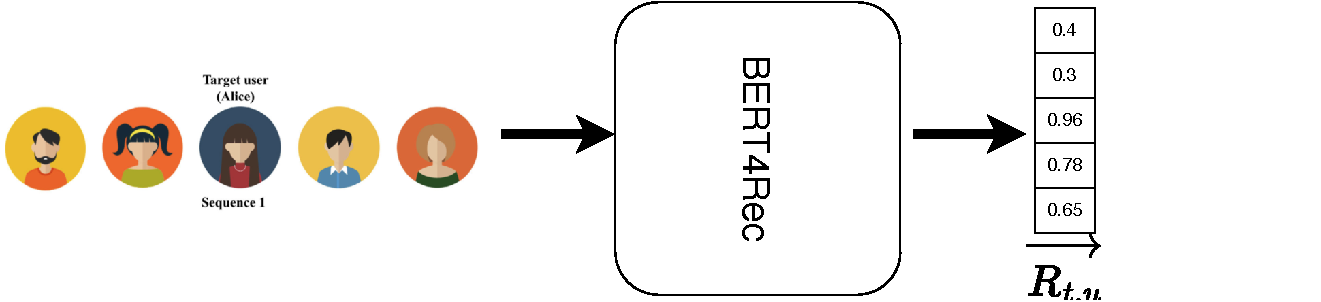
\includegraphics[width=0.4\textwidth]{images/CF_use_case.pdf}
        \caption{The adapted CBF-HybridBERT4Rec model on the left and the adapted CF-HybridBERT4Rec model on the right.}
        \label{fig:modelAdapt}
    \end{figure}

    \begin{equation}
        H(u) := (\{(x_i, t_j, s_k)| (x_i, t_j) \in R_{t,x}\}, \leq)
    \end{equation}
    \begin{equation}
        I(u) := (\{x_i|(x_i, t_j, s_k) \in H(u)\}, \leq)
    \end{equation}

    \begin{equation}
        u \in N \iff d_{u, t} = d_{u_m, t} \text{\,} \wedge (x, t) \in \{(x,t)|(x,t,s_k) \in H(u)\}
    \end{equation}

    \begin{algorithm}[ht!]
        \caption{HybridBERT4Rec in an E-Learning Setting}
        \begin{algorithmic}[1]
            \ForAll{$u_m \in U$}
                \State $r_{x,u_m} = \texttt{cbf\_hybridbert4rec}(H(u_m))$
                \ForAll{$(x,t) \in R_{t,x}$}
                    \State $r_{u, x} = \texttt{cf\_bert4rec}(u_m,t,x)$
                    \State $\hat{r}_{u,x} = \texttt{prediction\_layer}(r_{x,u}, r_{u,x})$
                \EndFor
            \EndFor
        \end{algorithmic}
    \end{algorithm}

    \FloatBarrier
    \subsection{Solving Evaluation}
    ABC
    \subsection{Remaining Possible Issues}
    ABC
    \section{Conclusion}
    ABC
%TC:ignore
%\clearpage %add new page for references
    \singlespacing
    \emergencystretch 3em
    \hfuzz 1px
    \printbibliography[heading=bibnumbered]

% \clearpage
% \begin{appendices}

% \section{Here go any appendices!}

% \end{appendices}

%TC:endignore
\end{document}